\chapter{Stand der Technik - Einführung in die Beacon-Technologie}
Der erste Teil in diesem Kapitel beschäftigt sich mit der Entstehungsgeschichte von iBeacons und nachfolgend mit deren Funktionsweise. Hier wird besonders auf die technischen Möglichkeiten der Technologie eingegangen. Im letzten Abschnitt wird erläutert, wo Beacon-Systeme zum Einstaz kommen und wie aktuelle Lösungsansätze für die Planung der dafür nötigen Infrastruktur aufgebaut sind. Anschließend wird aus den gegebenen Fähigkeiten der Beacons und der momentanen genutzten Fähigkeiten differenziert und eine Aussicht auf ein zukünftiges Konzept zu einer besseren Nutzung gegeben.

\section{Entwicklungsgeschichte}
Der Grundstein für die Beacon-Technologie legte die Firma Nokia im Jahre 2006. Damals entwickelte die Firma den neuen Standard \textit{Wibree} für die Funkübertragung,
%\begin{wrapfigure}{r}{5.3cm}
%\centering
%
\includegraphics[scale=0.07]{Bilder/BLE.png} 
%\caption{Offizielles Bluetooth Smart Logo \cite{BLElogo}}
%\label{BLElogo}
%\end{wrapfigure} 
der den alten Bluetooth-Standard ersetzen sollte. Mit der Neuentwicklung versprach man sich im Gegensatz zu Bluetooth einen geringeren Stromverbrauch und geringere Kosten, bei einem gleichbleibenden Kommunikationsbereich. Ab dem Jahr 2009 wurde der Bluetooth-Standard um Wibree ergänzt und erst unter den Bezeichnungen \textit{Ultra Low Power Bluetooth} (ULP) und dann später als \textit{Bluetooth Low Energy} (BLE) darin aufgenommen \cite{Wib2BLE} und anschließend als \textit{Bluetooth Smart} vermarktet. \par\bigskip
\begin{figure}[H]
\centering

\includegraphics[scale=0.07]{Bilder/BLE.png} 
\caption{Offizielles Bluetooth Smart Logo \cite{BLElogo}}
\label{BLElogo}
\end{figure}
%\vspace{2\baselineskip}
%\begin{wrapfigure}{l}{4cm}
%\centering
%
\includegraphics[scale=0.5]{Bilder/iBeaconLogo.png} 
%\caption{Offizielles iBeacon Logo \cite{iLogo}}
%\label{iLogo}
%\end{wrapfigure} 
Die Idee der Nutzung von Bluetooth Low Energy zur Indoor-Lokalisierung stammt dabei von der Firma Apple Inc. und wurde von ihr im Jahre 2013 auf der WWDC (Worldwide Developers Conference)\cite{Apple} unter dem Namen \textit{iBeacon} angekündigt. Obwohl zu dem Zeitpunkt noch kein fertiges Gerät zur Verfügung stand, wurde diese Technologie als Neuerung in Apples mobilen Betriebssystem iOS 7 vorgestellt. Jedoch verzichtet Apple seither auf die Produktion von iBeacons, was andere Unternehmen nutzen um selbst in den Markt einzusteigen. Deren Produkte unterstützen dabei zusätlich die mobilen Betriebssysteme Android ab Version 4.3, Windows Phone 8 und neue die neueste Version von Blackberries OS \cite{Bibel}. Somit wäre die Beacon-Technologie mittlerweile in über 99,5\% aller mobilen Geräte (Smartphones, Tablets, Smartwatches, etc.) weltweit nutzbar \cite{MobGerSt}.\par\bigskip
\begin{figure}[H]
\centering

\includegraphics[scale=0.5]{Bilder/iBeaconLogo.png} 
\caption{Offizielles iBeacon Logo \cite{iLogo}}
\label{iLogo}
\end{figure}

\newpage

\section{Aufbau und Funktionsweise von Beacons} 
\begin{wrapfigure}{r}{6cm}
\begin{flushright}
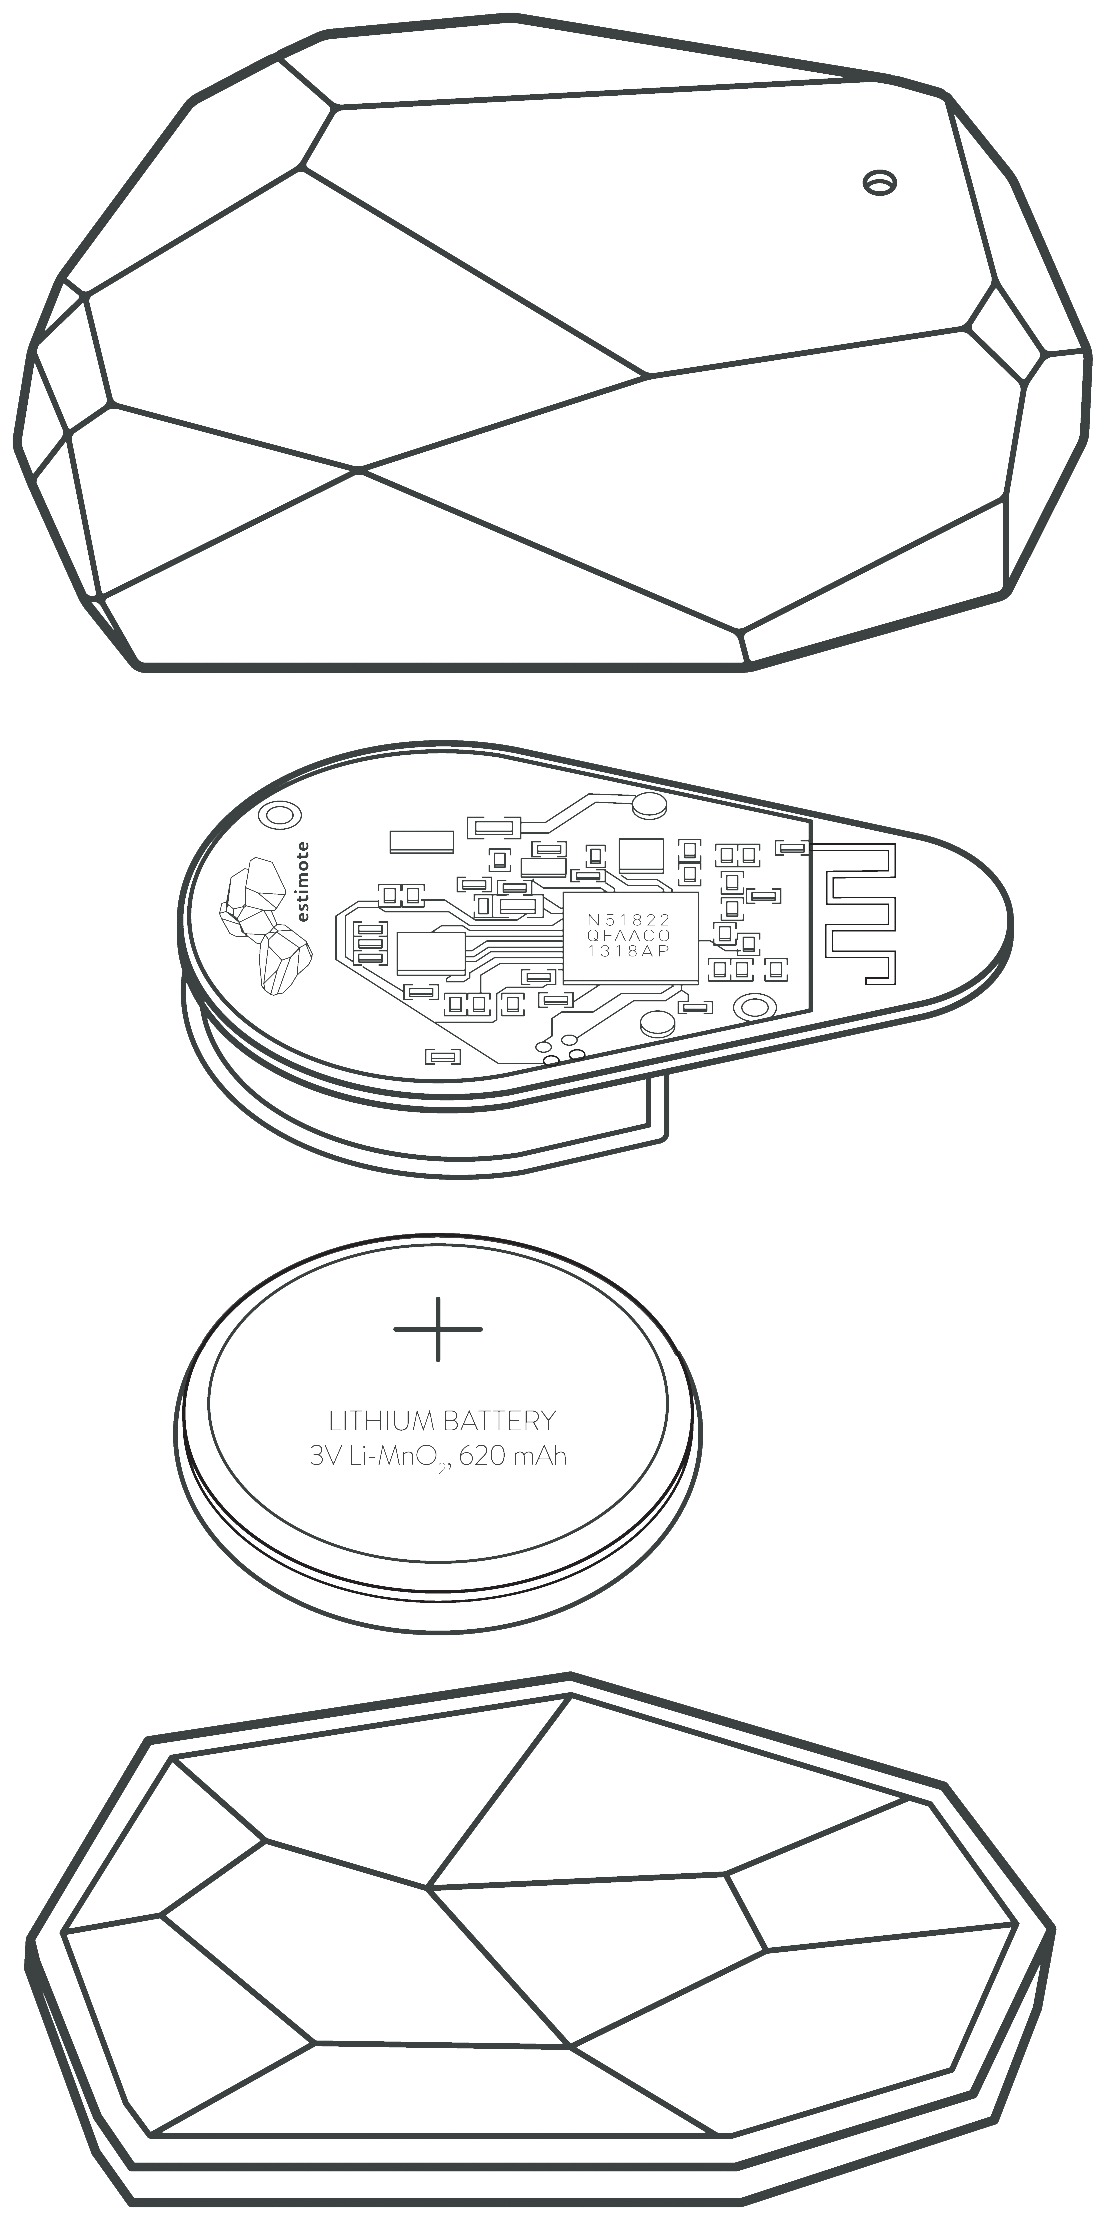
\includegraphics[scale=0.07]{Bilder/BeaconSchicht.png}
\caption{Explosionszeichnung Beacon \cite{BeaEx}}
\label{fig:BeaEx}
\begin{picture}(0,0)
\put(-150,177){Schutzhülle}
\put(-85,182){\line(1,0){25}}
\put(-150,137){Platine}
\put(-110,142){\line(1,0){50}}
\put(-150,100){Batterie}
\put(-100,105){\line(1,0){40}}
\put(-150,60){Silikonplatte}
\put(-80,65){\line(1,0){20}}
\end{picture}
\end{flushright}
\end{wrapfigure}
Die Grundbausteine eines Beacon sind in der rechten Abbildung \ref{fig:BeaEx} ersichtlich, in der ein \textit{Estimote Beacon} der Firma Estimote Inc. in seinen einzelnen Bestandteile dargestellt ist. Aufgrund der Verwendung der Estimote Beacons in dieser Arbeit, dienen hier zur Veranschaulichung. Zur Anbringung der Beacons dient die auf der Rückseite befindliche Silikonplatte. Diese haftet an nahezu jeder glatten Oberfläche und kann mithilfe von Wasser normal gereinigt werden. Somit können die Beacons im Grunde unbegrenzt angebracht und wieder abgenommen werden. Die äußere Schutzhülle besteht dabei ebenfalls aus einem Silikon und schützt die inneren Bauteile. Zu den inneren Komponenten gehören die Platine mit dem darauf verlöteten 32-Bit ARM Cortex M0 CPU mit 256 kB Flash-Speicher und dem 2,4 GHz BLE-Sendemodul, einer Antenne und eine Knopfbatterie zur autarken Stromversorgung. Die Beacons haben eine variable Sendeleistung von 4dBm bis -30dBm (entspricht einer Leistung von 2,512 bis 0.001 Milliwatt) und übertragen ihre Daten in Intervallen von 50 bis 0,5 Hertz. Die Kommunikation verläuft dabei bidirektional, d.h. vom Beacon zum Empfangsgerät und zurück. Während die Kommunikation von Beacon zu mobilen Gerät dazu dient, die Lokalisierung des Gerätes zu ermöglichen, dient die Kommunikation vom Smartphone, Tablet, etc. zum Beacon zur Überprüfung des Betriebszustandes und zur Programmierung der Beacons. \\ \\
Die bei der Signalübertragung verwendete Protokoll-Architektur Bluetooth Low Energy sendet dabei im 2,4 Ghz Band, welches ebenfalls von den Protokollen 802.11 ac/a/b/g/n, älteren Bluetooth-Standards, ZigBee, NFC, etc. genutzt wird. Eine kleine Übersicht zu den einzelnen Varianten und deren Eigenschaften findet sich im Anhang in Bild \ref{fig:FUE}. Die Vorteile vom 2,4 Ghz Band gegenüber anderen Frequenzbändern ergeben sich aus einer großen Reichweite der Funksignale und einer geringen Größe der Antenne für deren Erzeugung. Jedoch besitzt dieses Band auch gewisse Nachteile, die bei der Auslegung von Beacon-Konfiguartionen beachtet werden müssen. Die Verwendung des Protokolls im 2,4 Ghz Band ist dabei historisch bedingt und nahezu alternativlos, da sie zu den ISM-Bändern \cite{BuNet} zählt und nur diese somit frei nutzbar sind. Durch die Benutzung des 2,4 Ghz Bandes für die Datenübertragungen in WLAN oder Bluetooth treten bei vermehrter Nuztung des Bandes leicht Störungen in den Übertragungen auf. Somit hängt die Qualität der Signale und schlussendlich auch die Lokalisierungsgenauigkeit an der lokalen Auslastung des 2,4 Ghz Bandes. Weitere störende Faktoren für die Signalqualität  können auch physische Objekte haben, die sich zwischen Sender und Empfänger befinden. In den Bildern ... und ... wird dies einmal dargestellt. Denn durch die physikalischen Eigenschaften des 2,4 Ghz Bandes werden die Funksignale durch Materialien wie Wasser und Stahl besonders gut absorbiert. Da die meisten Gebäude aus Stahlbeton gebaut sind und der menschliche Körper aus einem großen Anteil aus Wasser besteht, wirken sich diese Umstände besonders stark auf die Qualität der Signale und am Ende auf die Anwendung der BLE-Technik für die Lokalisierung von Menschen in Gebäuden aus. Jedoch sei dies nur am Rande erwähnt und würde unter zusätzlicher Betrachtung dieser Aspekten nur den zeitlichen Rahmen dieser Arbeit sprengen. \\ \\
\begin{figure}[H]
$\begin{minipage}[b]{7cm}
\centering
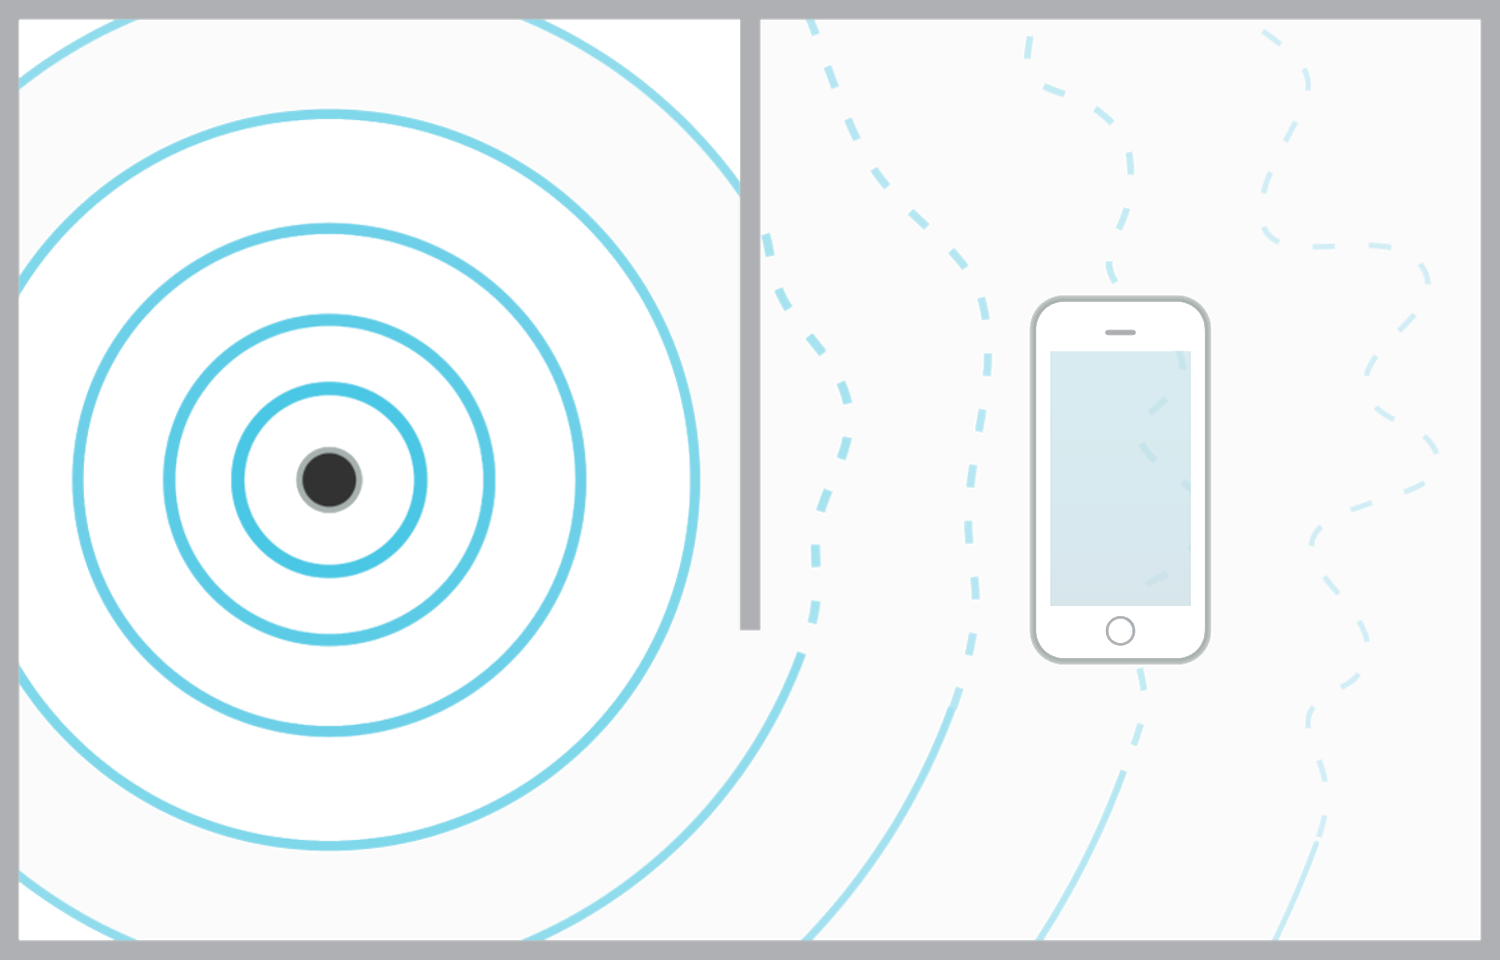
\includegraphics[scale=0.13]{Bilder/Wand.png} 
\caption{Signalschwächung durch Objekte, zB. Wände \cite{GSwiB}}
\label{fig:Wand}
\end{minipage}
\hspace{3cm}
\begin{minipage}[b]{7cm}
\centering
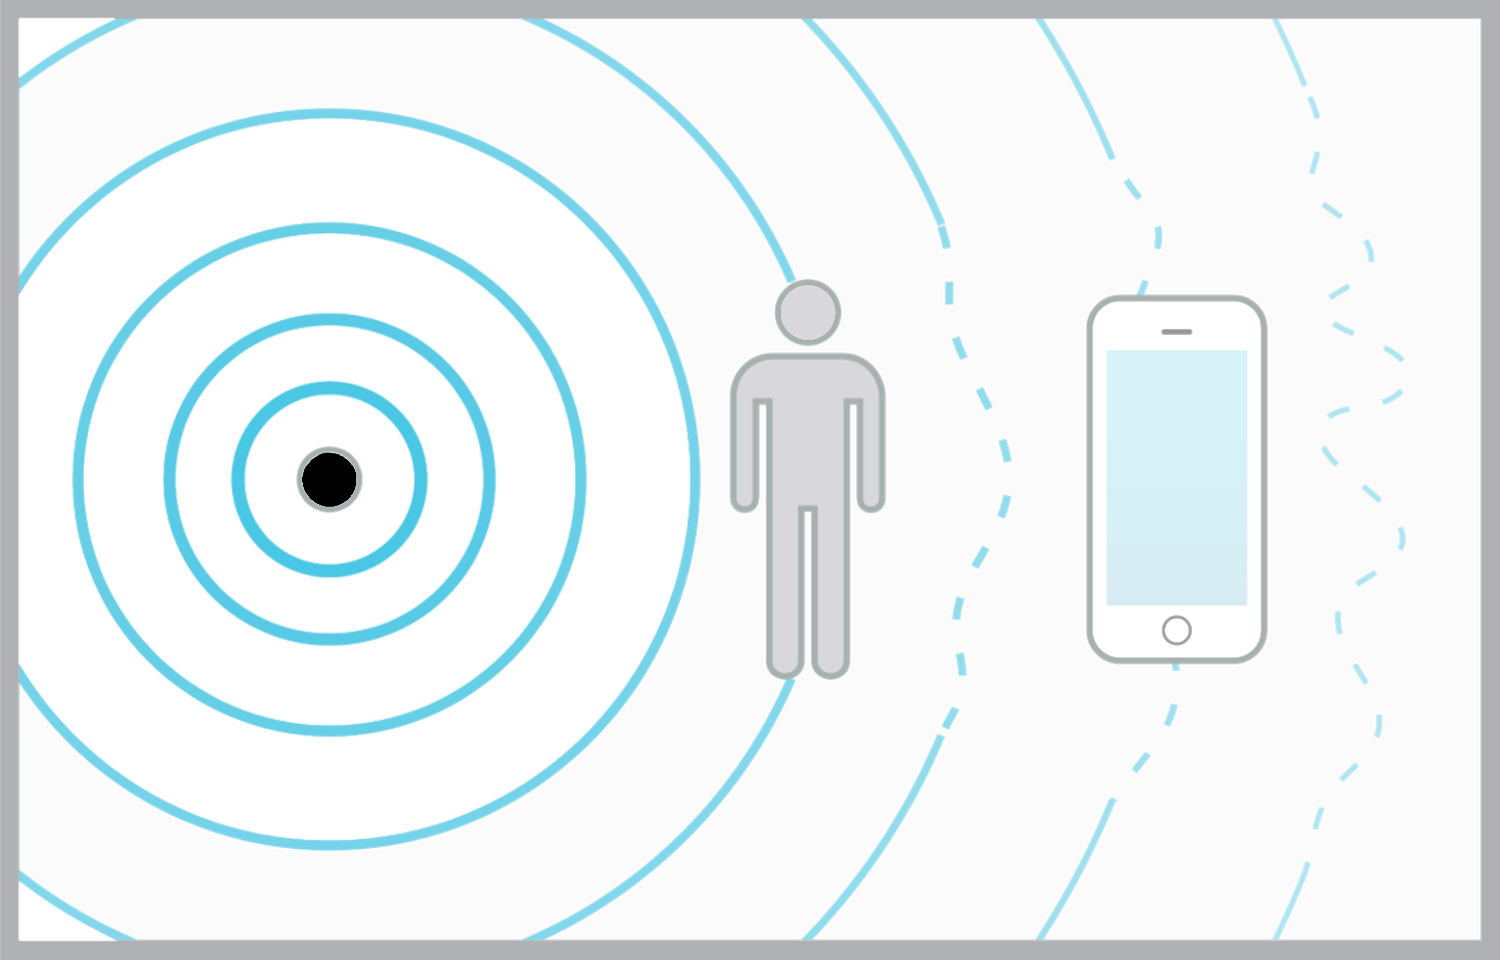
\includegraphics[scale=0.13]{Bilder/Hand.png} 
\caption{Körper von Menschen blockieren zusätzlich die Signale \cite{GSwiB}}
\label{fig:Hand}
\end{minipage}$
\end{figure}
Die Daten die bei der Kommunikation übertragen werden sind dabei essentiell für die Positionsbestimmung von Objekten und bestehen aus einer:
\begin{itemize}
\item Identifikationsnummer (Länge von 16 Bytes)
\item eingestellten Sendeleistung (2 Bytes)
\item zusätzlichen Information, beschrieben als Major und Minor (jeweils 2 Bytes)
\end{itemize}
Mit der Identifikationsnummer kann zwischen den einzelnen Beacons unterschieden werden, wodurch erst die Möglichkeit einer Lokalisierung entsteht. Denn die Technik setzt voraus, dass die Identitäten der Beacons in einer Datenbank mit Positionsangabe in einem Gebäude hinterlegt sind. Beim Empfang eines gültigen Signals wird der Beacon in der Datenbank gesucht und anschließend die Distanz von Empfangsgerät und Beacon berechnet. Die Berechnung findet auf der Grundlage eines Ausbreitungsmodells von Signalen in Abhängigkeit zur eingestellten Sendeleistung des Beacons statt, in der die empfangene Signalstärke als RSSI-Wert interpretiert  und dadurch eine Distanz geschätzt wird. Die Modelle der Hersteller sind typischerweise nicht frei zugänglich, deswegen sie auch hier nicht vorgestellt werden. Die als zusätzlichen Informationen gekennzeichneten Daten sind eine Erweiterung der Identifikationsnummer und bieten lediglich einen Komfort für die Entwicklung der Datenbanken. Im nächsten Abschnitt wird dies in Tabelle ... noch einmal veranschaulicht.\\ \\  

%%%%%%%%%%%->
Zur Entwicklung dient die SDK ..., sie ermöglicht ..., Firmware der Beacons ermöglicht Anpassung folgender Einstellungen:
\begin{itemize}
\item Identifikationsnummer
\item eingestellte Signalstärke
\item Sendeintervall
\item zusätzliche Informationen
\end{itemize}
%%%%%%%%%%<-

%\section{Verwendungsszenarien}
% Unterscheidung der Konzepte für die Beacon-Nutzung in Micro-Lakalisierung und Kontext bezogene Interaktionen (Wo ist wer?, usw.)
%Heute und morgen.
% Momentan nur willkürliche Plazierung von Beacons, kein Konzept, keine Vereinfachungen, keine Validierung, keine Optimierung
% 
% Momentan nur 3 stufiges Verfahren um Position anzugeben (near, middle, far)
%
%Der Bedarf an einer innerräumlichen Ortung ist dort vorhanden, wo es für den Besucher schwer ist sich zu orientieren. Diese können sein: Flugplätze, Einkaufszentren und Messehallen. Das Ziel ist es nun den Besuchern dieser Einrichtungen ein ähnliches System bereit zu stellen, wie sie es von den Verkehrswegen her kennen. Es soll mithilfe mobiler Geräte (z.B. Smartphones) lokalisieren und gegebenenfalls durch das Gebäude navigieren möchte, wie er es von den Verkehrswegen her gewohnt ist.
%
%Denn in großen Gebieten, wie z.B. Einkaufshäuser, Lagerhallen und Flughäfen braucht man Hunderte von iBeacons, um die gesamte Fläche zu 100 Prozent abzudecken. Im Idealfall kann ich später in Matlab noch Gebiete einpflegen, an der die Karte nach Regionen aufgeteilt wird, in denen die Genauigkeit der Lokalisierung eingestellt werden kann. Damit ließe sich Robotergestützt ein Gebiet abfahren, in denen Vorschläge für die Positionierung von iBeacons anhand eines Optimierungsalgorithmusses generiert werden. Hierbei ließe sich wunderschön eine Pareto-Front bilden, die aus Anzahl von iBeacons und Genauigkeit pro Region Positionierungsvorschläge entwirft. Je nach Kundenwunsch. ROTER FADEN ZU MEINER ARBEIT!
%
%Hier kann angesprochen werden das wir ein adaptives Verfahren entwickeln wollen, denn viele bisherige Systeme bieten lediglich ein Landmarkenssystem oder ein Positionierungssystem. Mit den Beacons soll beides möglich sei und je nach Kundenwunsch anpassbar werden.
%
% Hier die Tabelle aus dem Anhang
%
% 







